% Chapter 2

\chapter{\uppercase{Literature Survey}} % Main chapter title
\label{ch:survey} % For referencing

\begin{spacing}{1.5} 
\begin{sloppypar}
\section{AUTONOMOUS DRIVING}
Autonomous Driving (AD) refers to the technology of making the vehicle capable of sensing the surrounding environment and operating without human intervention or involvement. Intelligent Vehicles (IV) refers to a vehicle that owns the above technology to enable partial or fully automated functions. \cite{chen2023milestones}

AD can be categorized as 3 modules:
\begin{itemize}
    \item Perception
    \item Planning
    \item Control
\end{itemize}

The Society of Automotive Engineers (SAE) provides a taxonomy with detailed definitions of vehicle driving automation systems. There are 6 levels, they are:
\begin{itemize}
    \item Level 0 (L0): No automation
    \item Level 1 (L1): Driver Assistance
    \item Level 2 (L2): Partial Driving Automation
    \item Level 3 (L3): Conditional Driving Automation
    \item Level 4 (L4): High Driving Automation
    \item Level 5 (L5): Full Driving Automation
\end{itemize}
% insert architecture here
\subsection{Perception}
The perception of IVs is the first and the foundational step which determines the performance of the next stages. The perception is done using sensors such as Radar, cameras, GNSS, Lidar, Ultrasonic, Lidar, etc. To reduce the probability of failure and uncertain variables intervening, multiple different sensors are generally used. 

\subsubsection{Lidar}
They support high resolution 3D point cloud, Larger and wider sensing range, Accurate object and distance detection and robust to lightning but have high cost, poor performance in harsh weather and produce a large amount of data. The Figure \ref{fig:lidar} shows the newest technology in Lidar sensor: silicone-based Lidar sensors. Silicone based Lidar sensor reduce the volume of the conventional Lidar sensor and achieve a monolith integration. This removes the moving parts of the conventional Lidar sensors and realises solid-state beam steering \cite{hu2023advances}. 

\begin{figure}[h]
\begin{center}
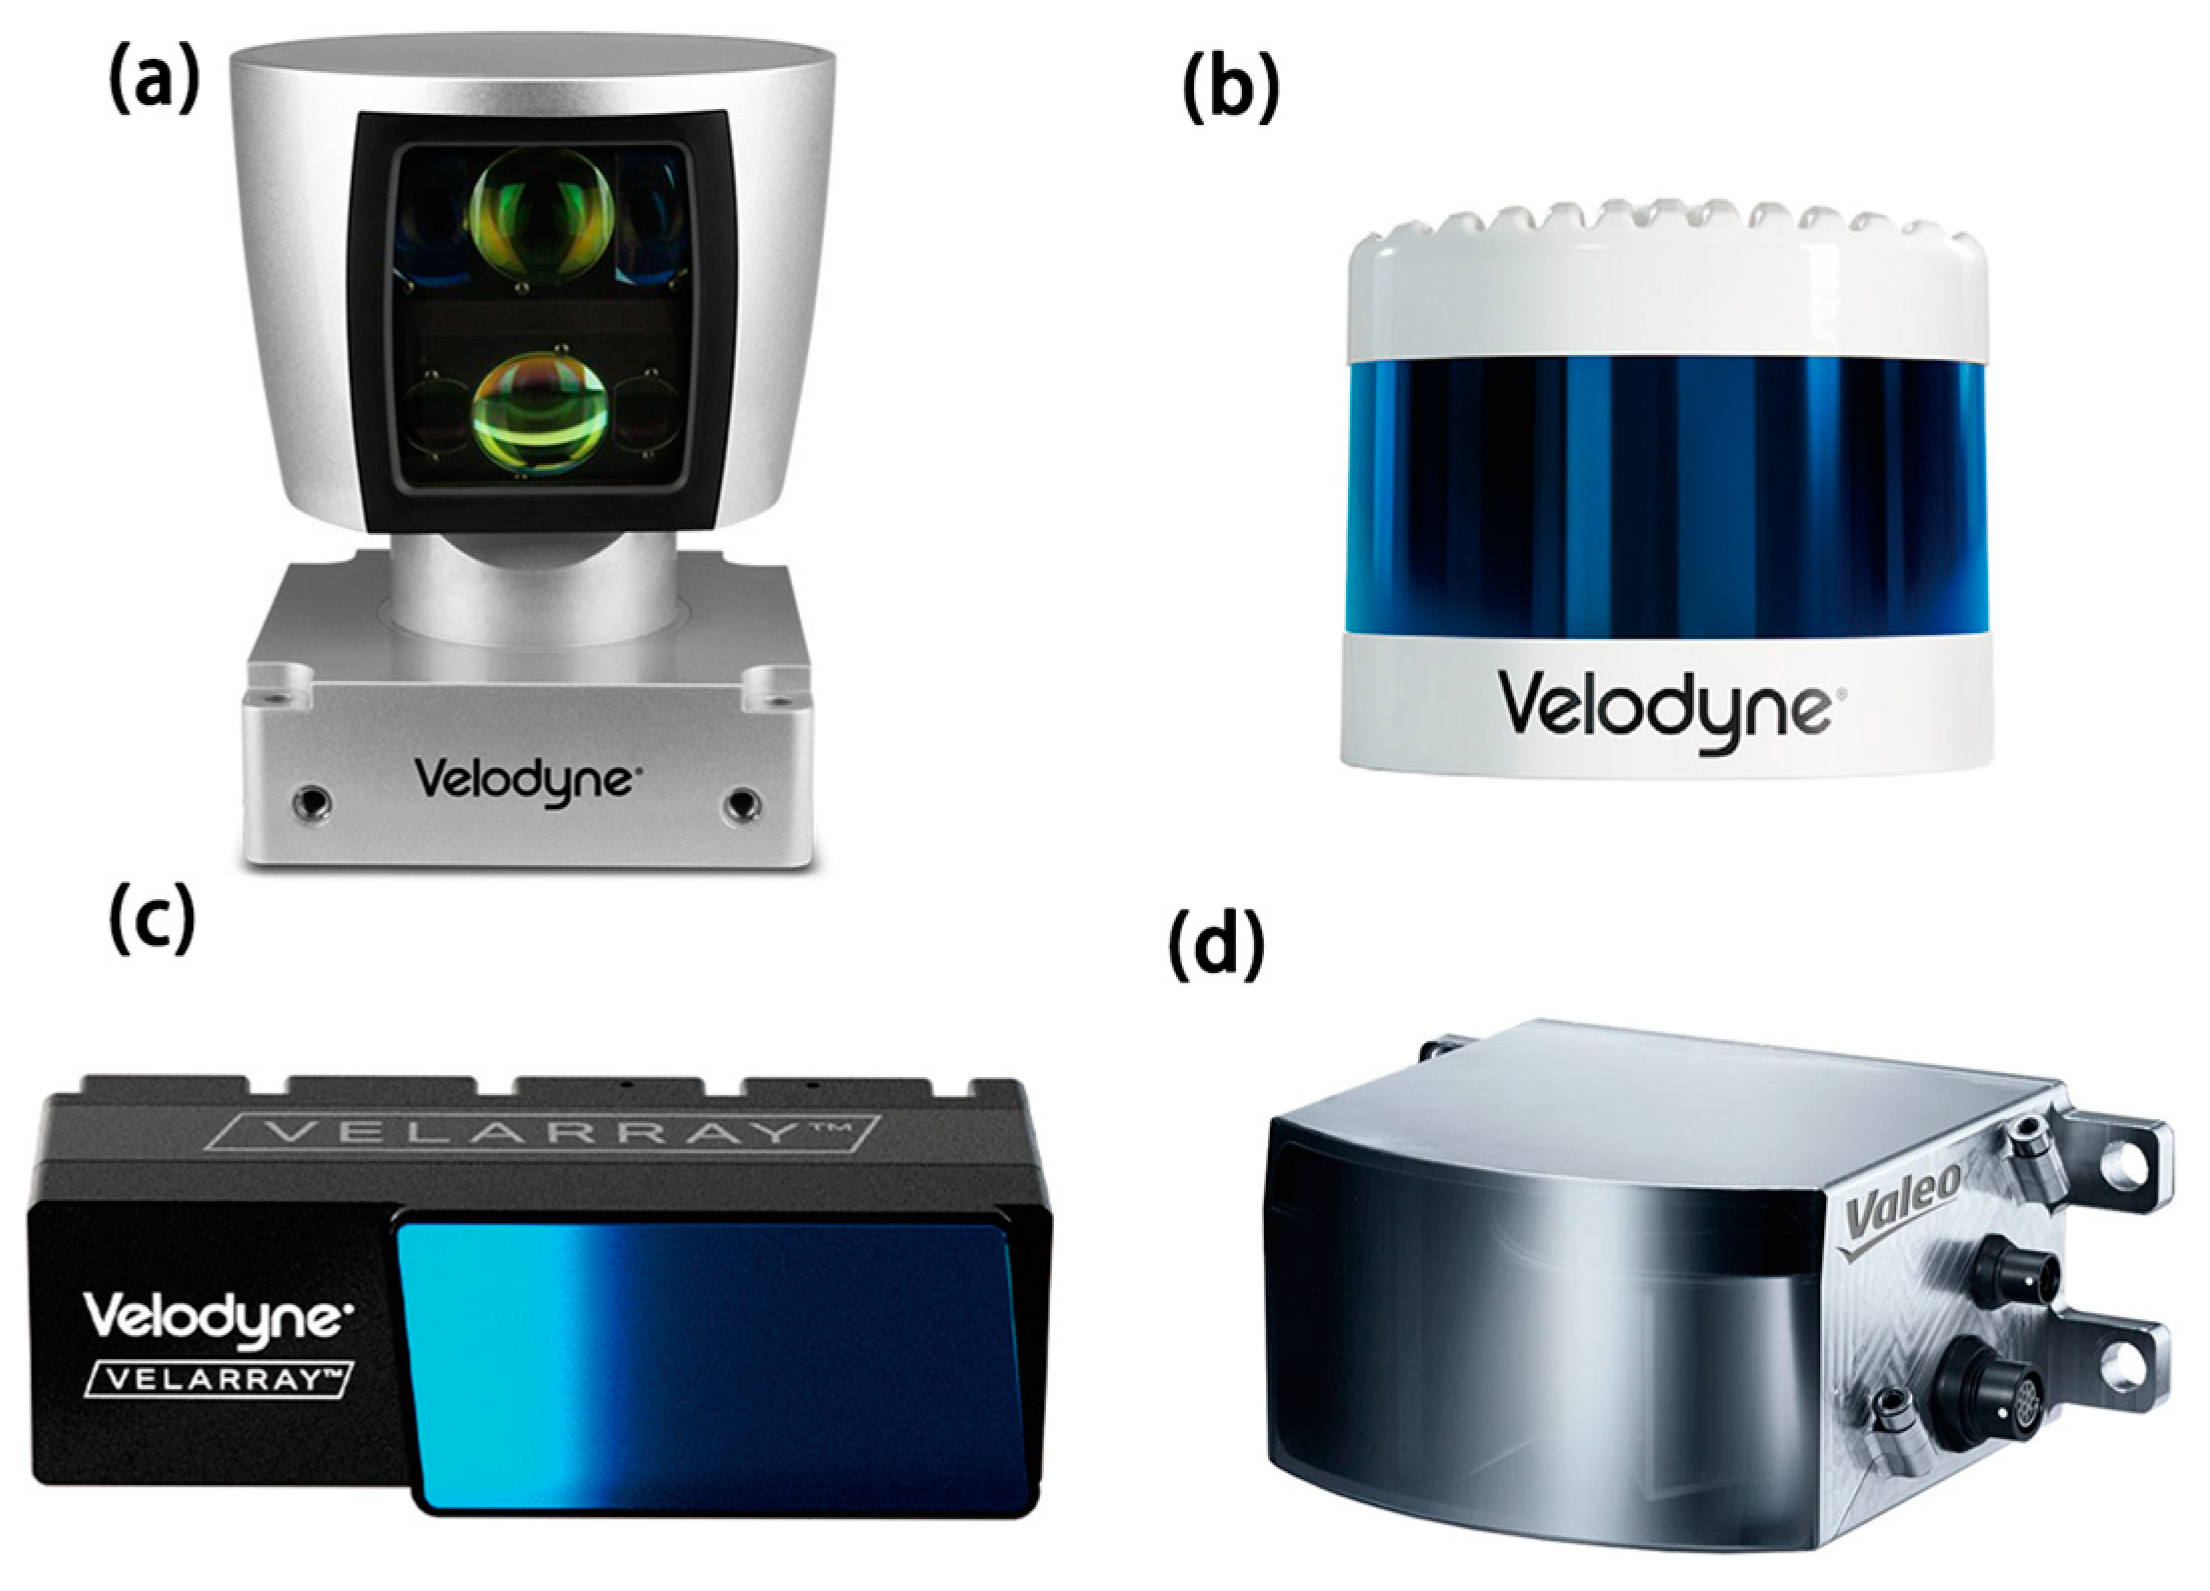
\includegraphics[scale=0.1]{2/lidar_Sensor.png}
\caption{Silicone-based Integrated Lidar Sensors in Intelligent Vehicles}
\label{fig:lidar}
\end{center}
\end{figure}

\subsubsection{Camera}
They are cost effective, support visual recognition and texture extraction but are easily affected by real world non-ideal environmental variables such as lighting and weather.

Multi-Object Tracking (MOT), an essential step in AD perception task, can be achieved by multiple cameras alone. Although, in practice, they are combined with Lidar and other sensors for SOTA performance. In the paper \cite{pereira2016self}, Akshay Rangesh et al utilize cameras and Lidar to achieve full-surround MOT using a modular design and also compares the results of different configurations such as number of cameras and positioning of cameras. Figure \ref{fig:camera} shows the full-surrond MOT using cameras. 

\begin{figure}[h]
\begin{center}
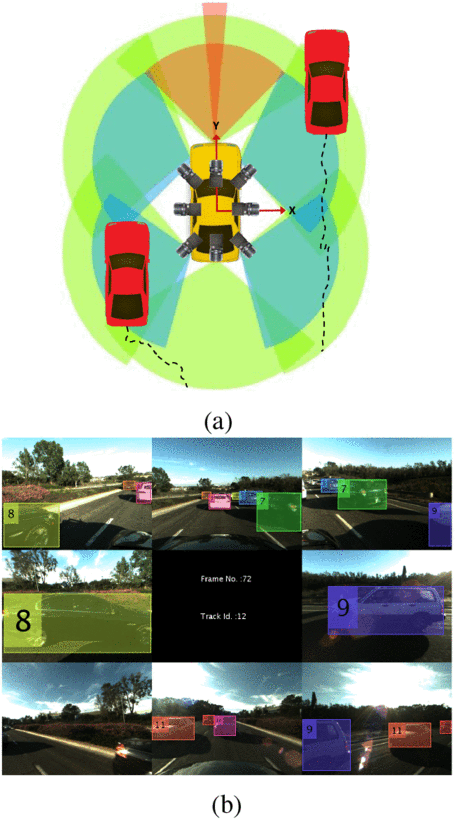
\includegraphics[scale=0.5]{2/camera.png}
\caption{Full-surround MOT using Cameras in Intelligent Vehicles}
\label{fig:camera}
\end{center}
\end{figure}
\subsubsection{Radar}
They support extreme long sensing range, are resilient to various external conditions but produce to little of data and cannot produce distinguishing features for targets.

Automotive radar have become more prominent due to its recent advancements in the radio-frequency (RF) CMOS technology that allows high-level radar on-chip integration. This lowers the cost of radar for mass production for consumers. But a disadvantage of mass produced consumer level radars are that they do no produce high spatial resolution. This can be mitigated by the multiple-input, multiple-output (MIMO) and cognitive approaches as discussed in this paper \cite{bilik2019rise}. Figure shows \ref{fig:radars} Radars using in Intelligent Vehicles. 

\begin{figure}[h]
\begin{center}
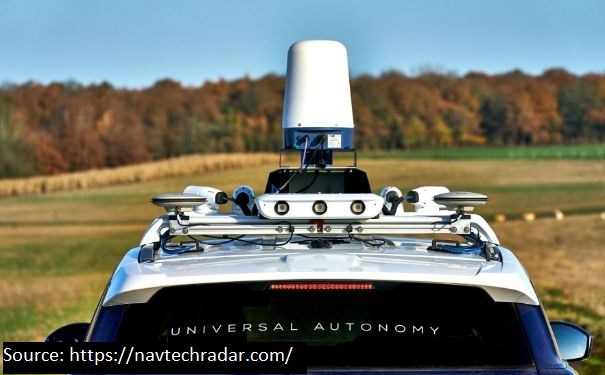
\includegraphics[scale=0.7]{2/radar.jpg}
\caption{Radars in Intelligent Vehicles}
\label{fig:radars}
\end{center}
\end{figure}

\subsubsection{GNSS}
They cost low, stable but have low accuracy, slow update frequency and require unobstructed view.

Modern Global Navigation Satellite Systems (GNSS) consists of four independent gloval satellite constellations delivering modernized signals at multiple civil frequencies. New ground monitoring infrastructure, mathematical models and internet services correct for errors in the GNSS signals at continent scale. Mass produced automotive grade receiver chipsets are available at low cost, size, weight and power (CSWaP). GNSS delivers better than lane-level accuracte localization with 99.99999\% integrity with over 95\% availability according to this paper \cite{joubert2020developments}. 
% \subsubsection{Ultrasound}
% They are Low cost, High accuracy for close range and resilient to adverse weather conditions but can only detect for short-ranges and don't work in high speeds.


\subsection{Planning}

Data-driven autonomous driving systems are characterized as modular tasks in a sequential order: Perception, Prediction and Planning. There exists standalone models for each task or one model with multiple different heads for each tasks. Yihan Hu et al \cite{hu2023planning} argue that all resources should be concentrated on the planning task as to not waste any resources unnecessarily. They optimize perception and prediction modules to primarily benefit the task of planning of self-driving cars. Figure \ref{fig:planning} depicts 3 types of Autonomous Driving designs, they are a) Separate models for different tasks, b) Multi-task learning scheme shares a backbone with divided task heads, c) End-to-end paradigm unites modules in perception and prediction.

\begin{figure}[h]
\begin{center}
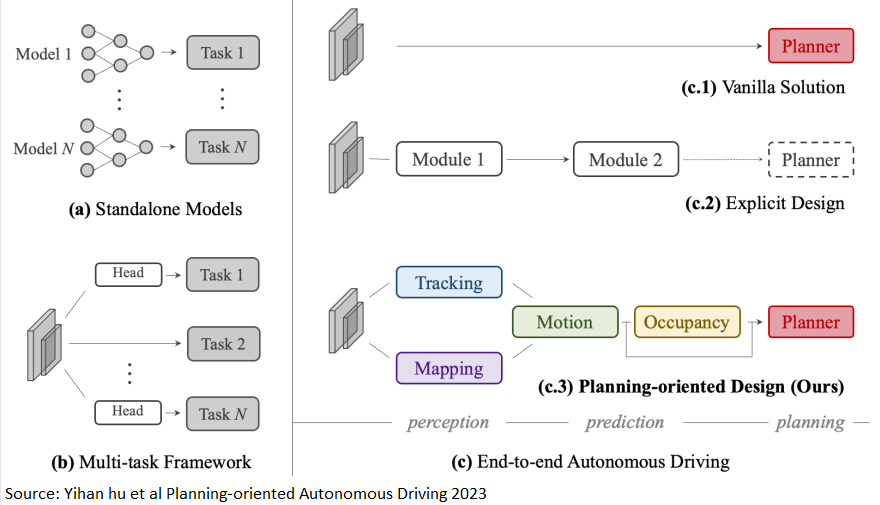
\includegraphics[scale=0.7]{2/hu2023Planning.png}
\caption{Planning-Oriented Autonomous Driving Design}
\label{fig:planning}
\end{center}
\end{figure}

 

\subsection{Control}
Vehicle control is an essential part of enhanced driver assistance. It includes tasks such as lateral stability control and driving at the limits for accident avoidance. There are two types of Motion control: 1) Longitudinal Vehicle Control which manages the acceleration of the vehicle through the vehicle's throttle and brake, and 2) Lateral Vehicle Control which controls the vehicle's position in the lane using the steering wheel. 

\subsubsection{Control Methodologies}
\textbf{PID Controller} or Proportional Integral Derivative Controller is a control loop mechanism employing feedback that is widely used in industrial control systems and variety of other applications requiring continuously modulated control according to Wikipedia.

In \textbf{Game-Theoretic Approaches} the vehicles are considered as players. Each player has a decision model which considers the game rules or traffic rules and other players to make it decisions. Since it considers what the other player will do, it is considered more reliable but has the drawback of being computationally intensive. 


\textbf{Fuzzy-Logic Control} is similar to PID controller, fuzzy-logic control does not require the mathematical model the mathematical model of the environment allowing the controller to adequately deal with nonlinear vehicle dynamics.

The principle of \textbf{MPC} or Model Predictive Control is to find a predictive motion solution over a longer horizon period by solving the problem at each sample tie and applying the first sequence of actions. In this way, MPC simulates a receding horizon control and changes the solution set to remain accurate to upcoming information.

\textbf{SMC} offers the capacity to adapt to unknown disturbances and matched uncertainties. 

\textbf{LPV Controller} is a linear controller and has been designed together with predictive control for lateral control and integrated system control.


\section{LARGE LANGUAGE MODEL}
LLMs are language models that are trained on large unsupervised datasets such as WebText. They are essential to the task of zero-shot task transfer for NLP task such as question and answering, machine translation, reading comprehension and summarization. Open-source of Open-access LLMs are model whose weights are publicly available for research and for some commercially also. LLMs are mad e up of transformers. GPT2 a predecessor of ChatGPT had size of 1.5 Billion parameters and was noted that it still didn't overfit meaning that it's performance can still be improved upon \cite{radford2019language}.
\subsection{OpenAI's GPT 3.5 And GPT 4}
OpenAI's ChatGPT-3.5, also known as GPT-3.5 Turbo, is a version of the Generative Pretrained Transformer (GPT) model that has been fine-tuned for chat applications. It is capable of understanding and generating natural language or code. This model was trained on an Azure AI supercomputing infrastructure and finished training in early 2022.
ChatGPT-3.5 Turbo has been optimized to perform better for specific use cases and run these custom models at scale. Early tests have shown that a fine-tuned version of GPT-3.5 Turbo can match, or even outperform, base GPT-4-level capabilities on certain narrow tasks. \cite{bahrini2023chatgpt}
% As for the reference paper, you can refer to the paper titled "ChatGPT: Applications, Opportunities, and Threats" submitted to arXiv.org on April 14, 2023. This paper provides a comprehensive examination of the applications, opportunities, and threats of ChatGPT in various domains. It also includes an experimental study comparing the performances of GPT-3.5 and GPT-4.

% \subsection{OpenAI's GPT 4}
\subsection{Llama And Llama2}
LLaMA and LLaMA 2 are collections of foundation language models developed by Meta AI. These models range in scale from 7 billion to 70 billion parameters.
LLaMA \cite{touvron2023llama} was trained on trillions of tokens using publicly available datasets exclusively. LLaMA-13B outperforms GPT-3 (175B) on most benchmarks, and LLaMA-65B is competitive with the best models, Chinchilla-70B and PaLM-540B.
LLaMA 2 \cite{touvron2023llama2} includes both pretrained and fine-tuned large language models (LLMs). The fine-tuned LLMs, called LLaMA 2-Chat, are optimized for dialogue use cases. LLaMA 2 outperforms other open-source chat models on most benchmarks.
These models are freely available for research and commercial use.

LLaMA introduces distinct innovations such as SwiGLU activation functions, rotary positional embeddings, root-mean-squared layer-normalization, and key-value caching. It also uses a zero-initialized attention mechanism with zero gating, which adaptively injects new instructional cues into LLaMA while effectively preserving its pre-trained knowledge.

\subsection{Mistral and Mixtral}
Mistral \cite{jiang2023mistral} is a 7-billion-parameter language model engineered for superior performance and efficiency. Mistral uses a Sliding Window Attention (SWA) mechanism. Each layer attends to the previous 4,096 hidden states. It also uses Grouped Query Attention (GQA), which allows for faster inference and lower cache size.
Mixtral is a Sparse Mixture of Experts model. Mixtral-8x7B outperforms GPT-3.5 using a technique called Mixture of Experts (MoE)
% \subsection{Mixtral}
% \subsection{OpenChat}

% \section{Data-driven IV}

% \subsection{Perception}
% \subsection{Planning}
% \subsection{Control}

\section{KNOWLEDGE DRIVEN DRIVING AGENTS USING LLM}
In this section, we will be looking at some recent papers that integrate LLMs to perform various autonomous driving task and give a review on how they do it. 
\pagebreak
\subsection{Working with Semantic Information}
To extract semantic information we use visual encoders. In Jinkyu Kim et. al. \cite{grounding} and Jinkyu Kim et. al. \cite{textual} the visual encoder is implemented using a Convolutional Neural Network.
Whereas Zhenhua Xu et. al. \cite{xu2023drivegpt4} uses a video tokenizer to take $N$ video frame. The tokenizer works by using a pretrained CLIP visual encoder to extract the features of $N$ input video frames. These tokens are then projected onto the text domain. Figure \ref{fig:driveGPT4} shows how this works.

Bu Jin et. al. \cite{jin2023adapt} also uses a video tokenizer but with Video Swin Transformer instead of CLIP to get the tokens.   

\begin{figure}[h]
\begin{center}
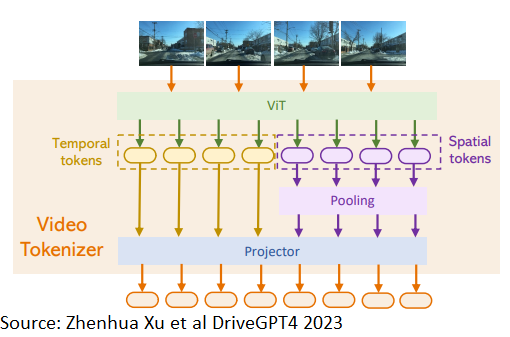
\includegraphics[scale=0.8]{2/DriveGPT4_1.png}
\caption{Architecture of Video Tokenizer}
\label{fig:driveGPT4}
\end{center}
\end{figure}

Zhenhua Xu et. al. \cite{xu2023drivegpt4} also use Llava (multimodal llm) and Yolov8 (real-time object detection) to generate prompts and give it to chatGPT to create a dataset for downstream task fine-tuning purpose. 

Long Chen et. al. \cite{chen2023driving} integrates numeric vector modality, a type of data frequently used in robotics to represent speed, actuator positions and distance measurements into the pretrained LLMs. This alleviates the problems of Visual Language Model's scaling problem. Figure shows the architecture of how this works.


\begin{figure}[h]
\begin{center}
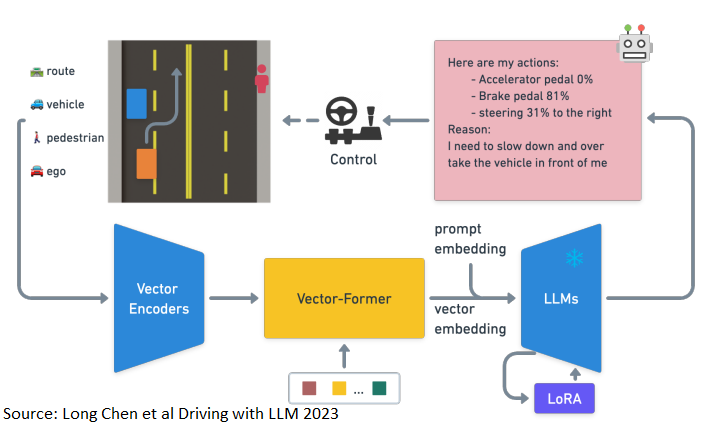
\includegraphics[scale=0.8]{2/vectorFusion.png}
\caption{Architecture with Vector Modality Instead of Visual Encoding}
\label{fig:vector}
\end{center}
\end{figure}


% \subsubsection{Multi-modal LLMs}


% There is an associated text encoder which encoders the text that describes the Image or video. 

\subsection{Autonomous Driving Tasks using LLMs}

In Licheng et. al. \cite{wen2023dilu}, an architecture for a knowledge-driven paradigm for Autonomous Driving System based on LLM that will interact with the environment to continuously evolve with a driver agent that recalls, reasons and reflects on it actions given a situation. The Figure \ref{fig:dilu} shows its architecture of a knowledge-driven driving agent using LLM.

\subsection{BDD-X Dataset}
Jinkyu Kim et. al. \cite{textual} uses Spatial, Temporal and Spatio-Temporal attention for vehicle control and explanation generation. It consists of 2 modules, 1) Vehicle Controller and 2) Explanation generator. The Figure \ref{fig:textual}

Jinkya Kim et. al. \cite{textual} includes the BDD-X dataset. It focuses on generating textual description and explanations such as the pair “Vehicle slows down” (description) and “Because it is approaching an intersection and the light is red” (explanation)". Figure \ref{fig:textual2} shows how the dataset is organized.  

\begin{figure}[h]
\begin{center}
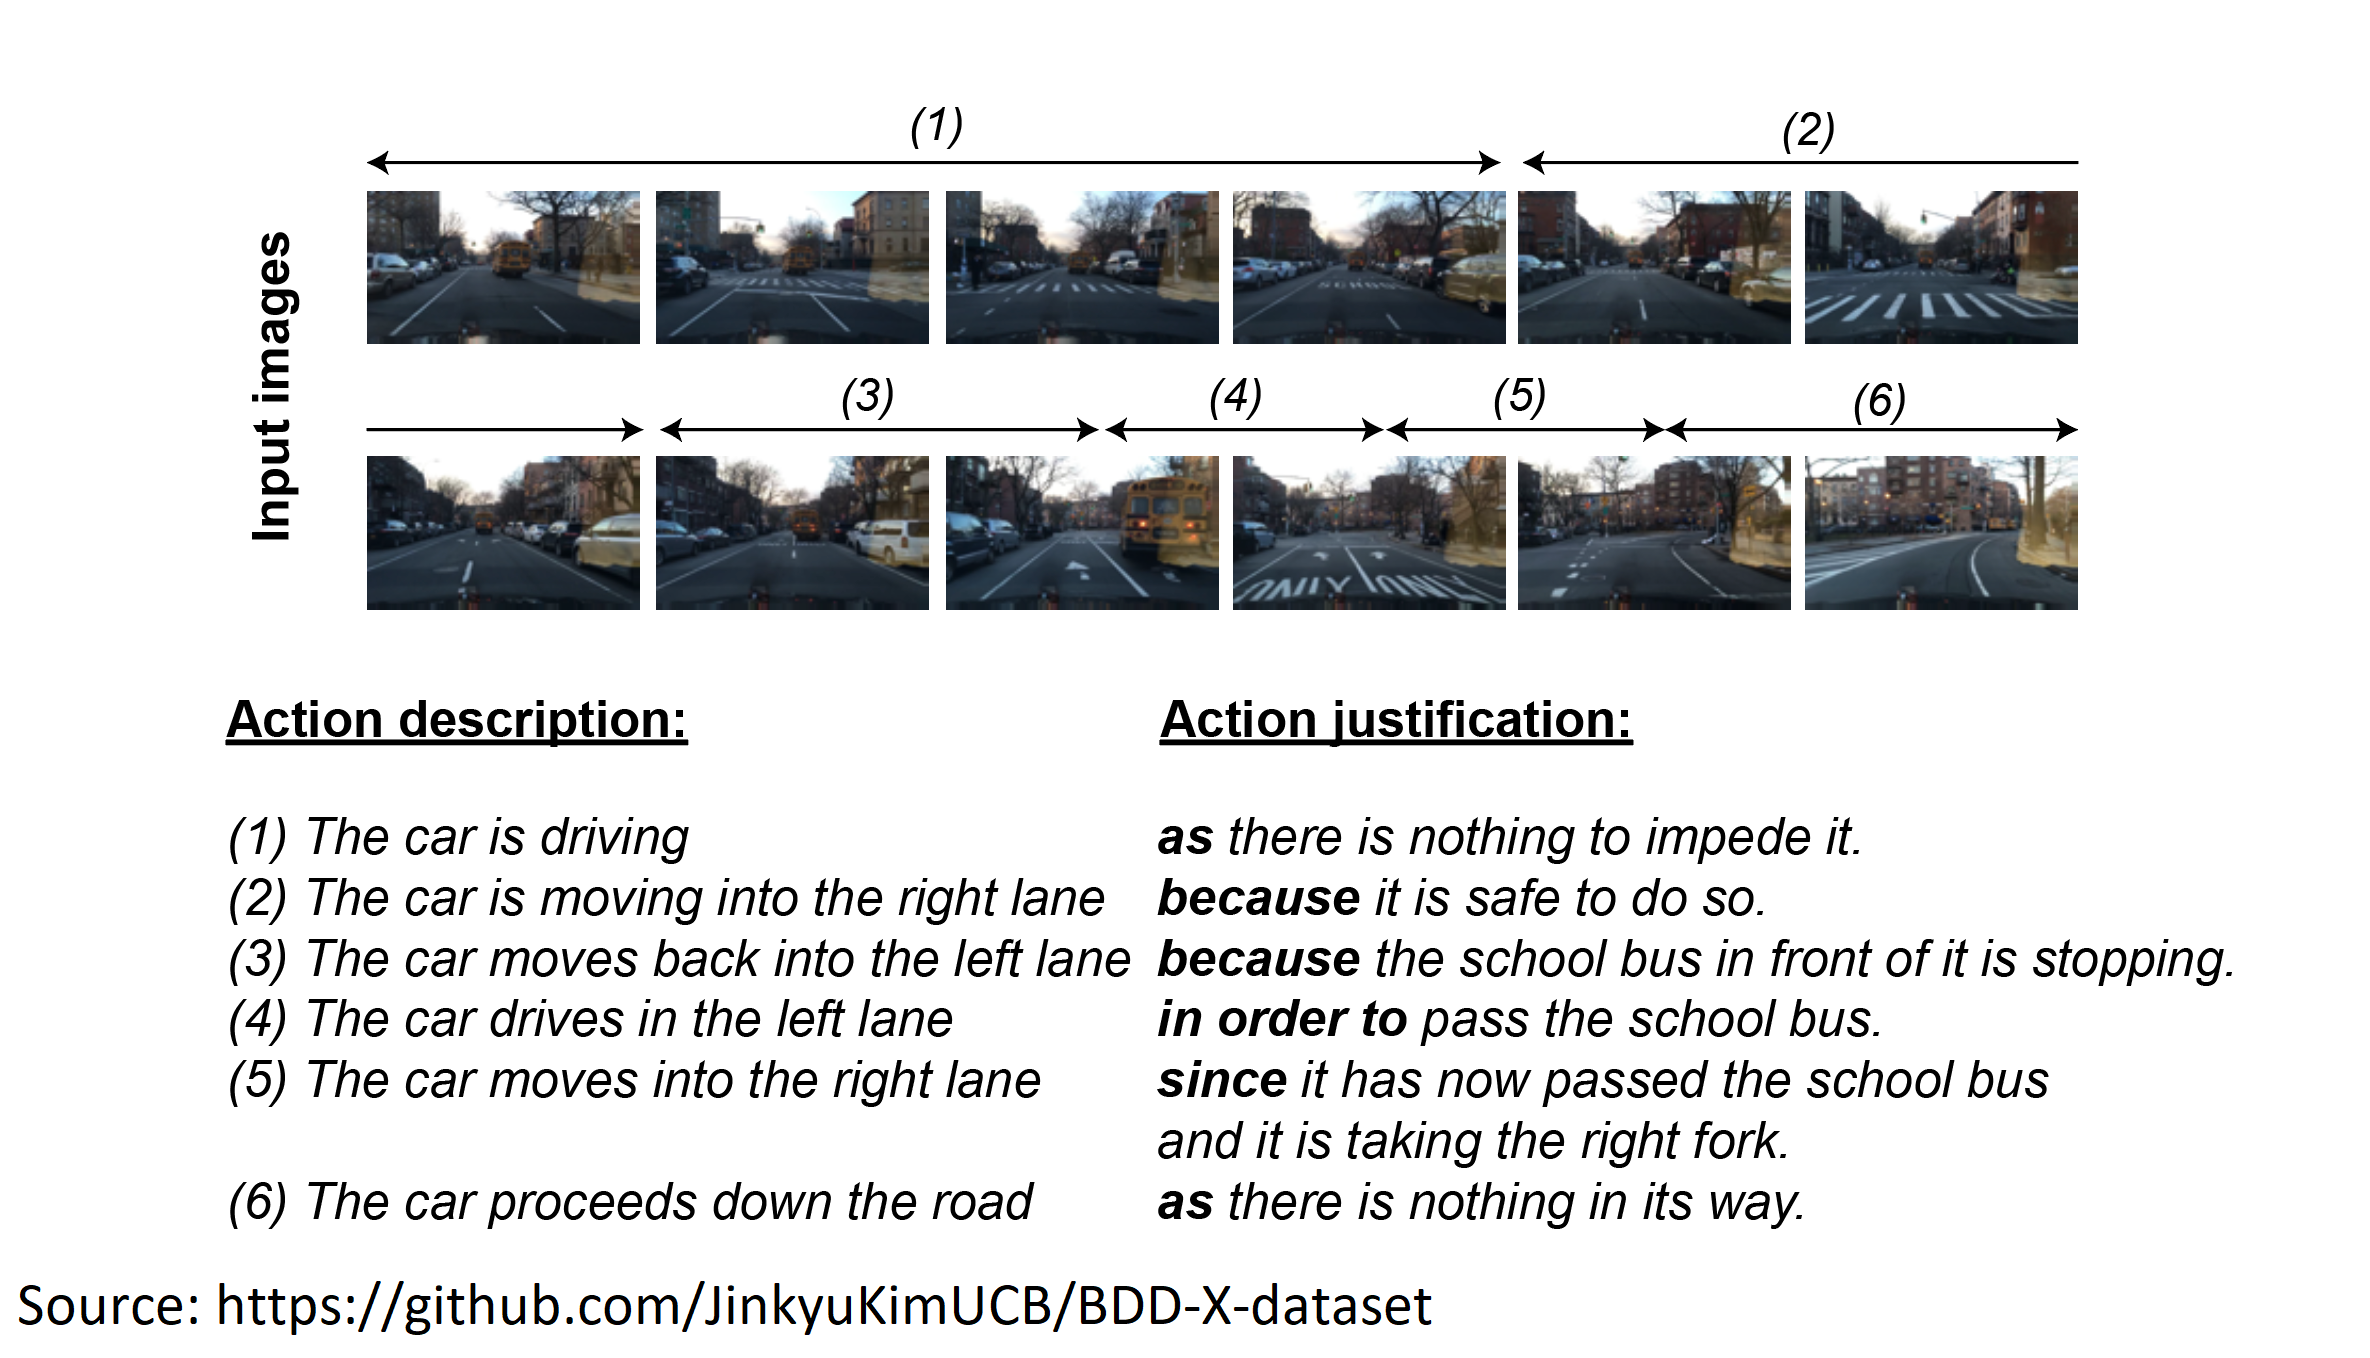
\includegraphics[scale=0.3]{2/textual_2.png}
\caption{BDD-X Dataset}
\label{fig:textual2}
\end{center}
\end{figure}

\begin{figure}[h]
\begin{center}
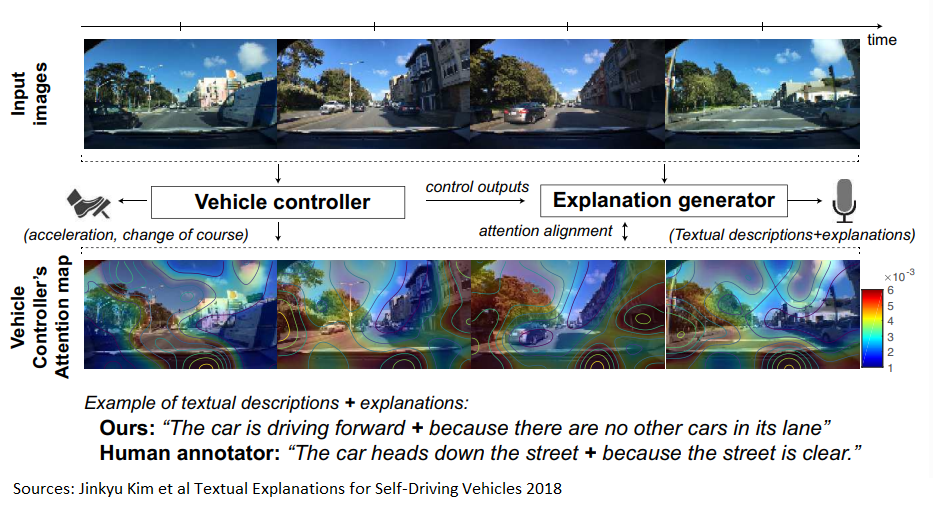
\includegraphics[scale=0.8]{2/textual_1.png}
\caption{Textual Explanations for Self-Driving Vehicles Overview}
\label{fig:textual}
\end{center}
\end{figure}

Bu Jin et. al. \cite{jin2023adapt} uses $T$ video frames as inputs (32 frames for best performance). It outputs are 1) control signal which is used to control the vehicle and 2) Text which consists of narration (what is happening?) and reasoning(why it is happening?). This work is similar to Jinkyu Kim et. al. \cite{textual} with few differences such as use of tranformers. The Figure \ref{fig:adapt} shows the architecture of Bu Jin et. al. \cite{jin2023adapt}.

\begin{figure}[h]
\begin{center}
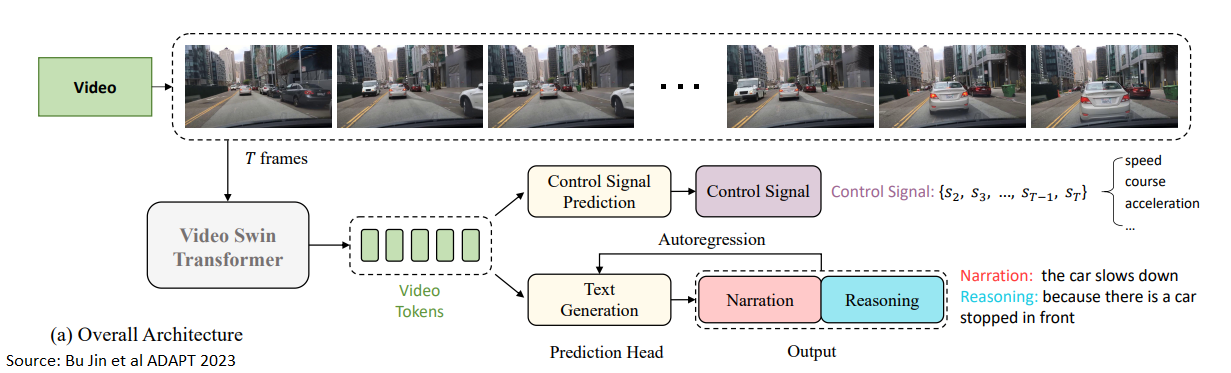
\includegraphics[scale=0.6]{2/ADAPT_1.png}
\caption{ADAPT Overview}
\label{fig:adapt}
\end{center}
\end{figure}

Zhenhua Xu et. al. \cite{xu2023drivegpt4} uses 8 video frames as inputs to predict the next viable actions to take as well as attain a reasonable understanding of its situation. Figure \ref{fig:driveGPT4_2} shows the work of Zhenhua Xu et. al. \cite{xu2023drivegpt4}.

\begin{figure}[h]
\begin{center}
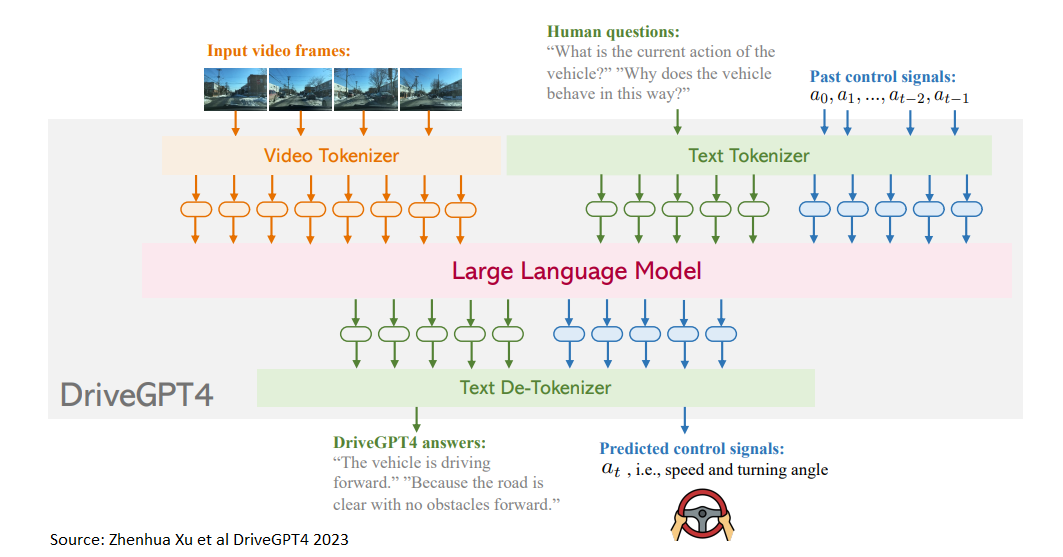
\includegraphics[scale=0.7]{2/DriveGPT4_2.png}
\caption{DriveGPT4 Overview}
\label{fig:driveGPT4_2}
\end{center}
\end{figure}


\begin{figure}[h]
\begin{center}
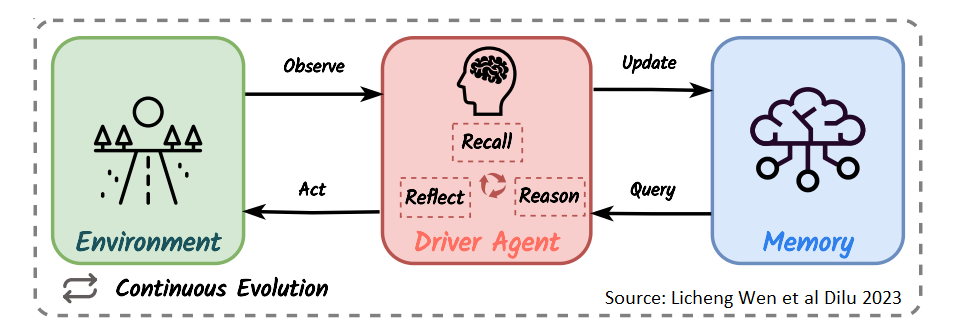
\includegraphics[scale=0.7]{2/Dilu_1.png}
\caption{A Knowledge-Driven Driving Agent Architecture using LLM}
\label{fig:dilu}
\end{center}
\end{figure}

This work is based on the Daocheng Fu et al \cite{fu2023drive}, GPT 3.5  observes its environment using perception tools and makes discrete decisions to control the ego vehicle. GPT 3.5 employs the ReAct strategy to plan actions and use tools to perceive its surroundings through a cycle of thought, action and observation. Figure \ref{fig:driving} shows the work of Doacheng Fu et al \cite{fu2023drive}.

\begin{figure}[h]
\begin{center}
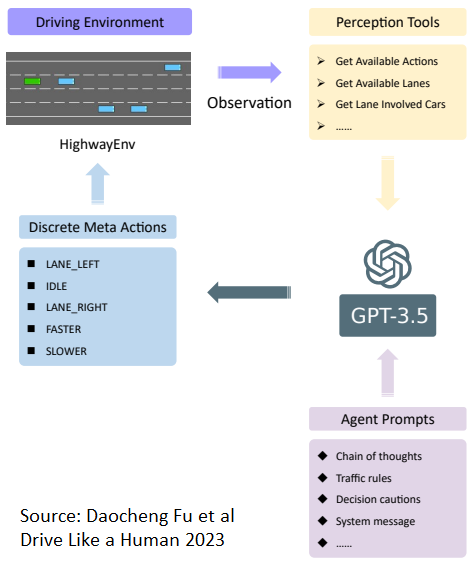
\includegraphics[scale=1.5]{2/DriveLikeHuman_1.png}
\caption{Driving like a Human}
\label{fig:driving}
\end{center}
\end{figure}
\end{sloppypar}
 \end{spacing}

 
